\chapter{需求建模 }
\section{数据流图}

    \textbf{注}:对于即时通讯系统,对数据的主要操作是传递数据、分发数据,而不存在独立出来的处理数据的过程。故数据流图的内容实为不多,仅用顶层数据流图足以展示全面,故0层、1层数据流图未再考虑。
\subsection{顶层数据流图}
% <Draw the Top-level DFD here>

% 在这里画出顶层数据流图

\begin{figure}[ht]
    \centering
    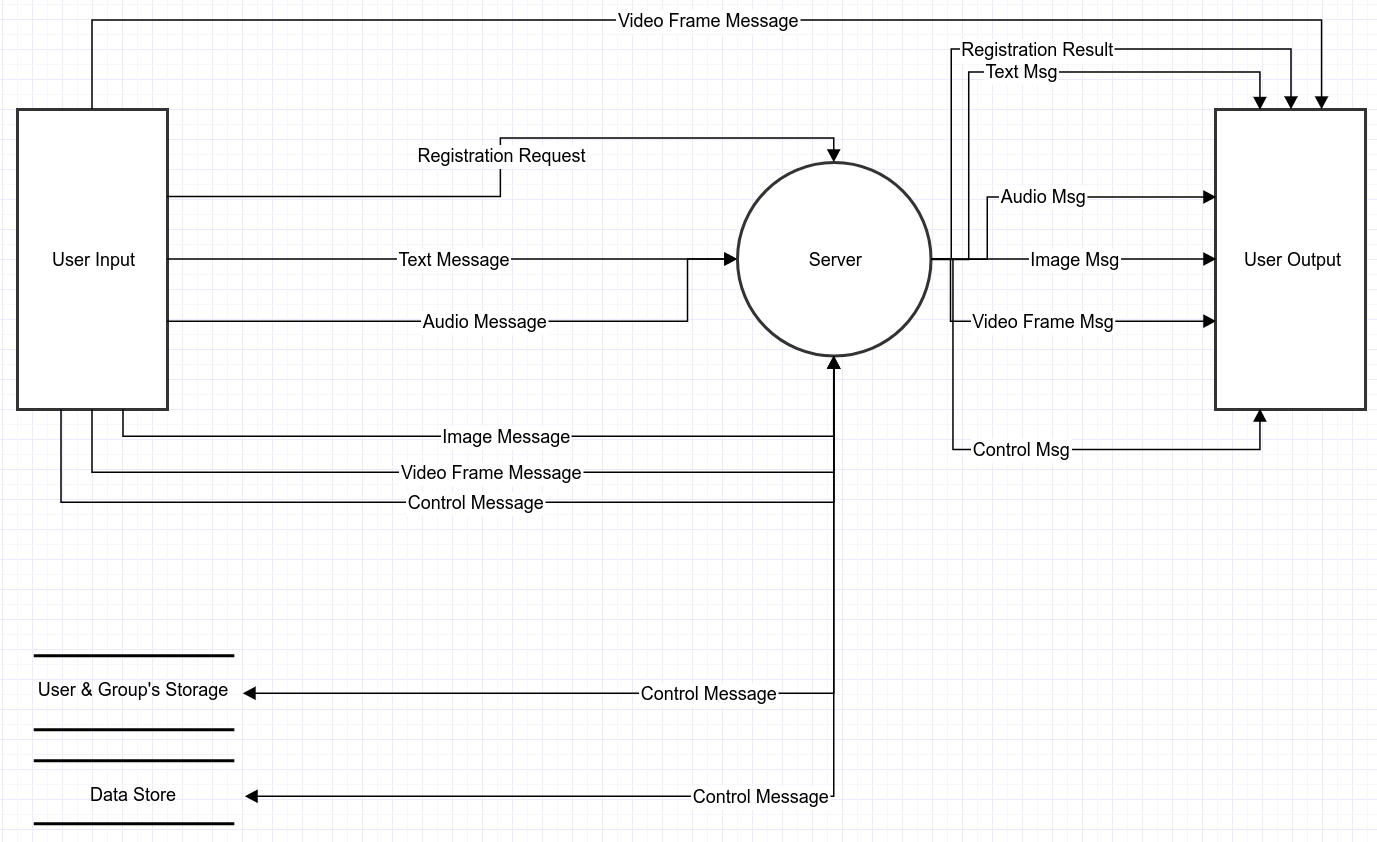
\includegraphics[width=15cm]{data_flow_diagram_high.png}
    \caption{顶层数据流图}\label{fig:figure1}
    
    \end{figure}

% \subsection{层数据流图}
% <Draw the Level-0 DFD here>

% 在这里画出0层数据流图

% \subsection{层数据流图}
% <Draw the Level-1 DFD here>

% 在这里画出1层数据流图

\section{数据字典}
\subsection{数据流说明}
\subsubsection{Registration Request 注册请求信息}
% <Title of  the data flow should accord with the one in data flow diagram, and the Data description notions should be used.  >

% 与数据流图中的名称一致,采用数据描述符号说明数据流的内容
这是由新注册用户所发出的注册请求信息,它包含了用户名,密码等基本信息,以及可选的用户资料(User Profile,如头像,性别,出生日期,所在地等)。

\subsubsection{Registration Result 注册结果信息}
这是返回给新注册用户的注册结果,它指出了注册是否成功,以及一串数字,它将作为该用户第二个用户ID。

\subsubsection{Text Message 文本消息}
这是由已登录用户向另一用户或群组所发出的文本消息。

\subsubsection{Audio Message 语音消息}
这是由已登录用户向另一用户或群组所发出的二进制编码的语音消息。

\subsubsection{Image Message 图片消息}
这是由已登录用户向另一用户或群组所发出的二进制编码的图片消息。

\subsubsection{Video Frame Message 视频帧消息}
这是由已登录用户在进行视频聊天时,不断发出的视频帧消息。\\
注:数据流图中存在两条视频帧消息的数据流,这表示视频帧可能会经过产品服务器的转发,也可能会直接从客户端由UDP协议传输到另一客户端。具体的选择会与当时的网络环境有关。

\subsubsection{Control Message 控制消息}
此类数据流包含多种功能的消息:如添加好友的确认消息、创建群组的命令,以及各种在产品实现中会用到的同步消息。
该类数据流中的有些会作用于另一客户端,有些会作用到服务器的数据库,使得用户、群组在服务器中的存储得以改变。

\subsection{数据存储说明}
\subsubsection{User/Group's Storage 用户和群组存储}
% <Title of  the data flow should accord with the one in data flow diagram, and the Data description notions should be used. The arrangement of the data in data store should also be described.>

% 与数据流图中的名称一致,采用数据描述符号说明数据流的内容,另外还需描述数据排列方式
这块存储区域存储了用户/群组本身的基本信息、用户资料,以及用户与用户之间的好友关系、用户与群组之间的关联。

\subsubsection{Data Store 其他数据存储}
这块存储区域存储了聊天过程中需要保存到云端的数据,如一定期限内的聊天记录。

\subsection{加工说明}
\subsubsection{Server 服务器处理模块}
% <Use natural language, Decision table/Decision tree and Pseudocode to describe how to process the data flow>

% 采用自然语言,判断表/判断树,伪码的形式描述对数据流进行处理的过程
加工各种消息的模块在实现中会十分繁杂,在此将它简化成单一的模块。

\begin{itemize}
    \item \textbf{注册请求(Registration Request)的处理}\\
    服务器会再次验证注册数据的合法性,这是为了防止恶意人员使用产品的API未经客户端的检查而定制自己的请求。\\
    当完成检查后,将输出(Registration Result)发送至用户。
    \item \textbf{各类用户会话消息(文本消息、语音)的处理}\\
    服务器会再次验证消息的完整性、鉴别真实性(通常由消息中的某些字段来鉴别),以及大小是否合适,这也是为了防止恶意人员使用爬虫,通过产品的API,未经客户端的检查而定制自己的请求。\\
    当完成检查后,执行一些必要的序列化操作,将数据以合适的格式发送到目标用户/群组。
    \item \textbf{各类控制消息的处理}\\
    服务器会鉴别控制消息的真实性,如果真实有效,则执行相应操作,将输出的更改存入相应的数据库。
\end{itemize}

